%%%%%%%%%%%%%%%%%%%%%%%%%%%%%%%%%%%%%%%%%%%%%%%%%%%%%%%%%%%%%%%%%%%%%%%%%%%%%
% Technical report, NeurIPS 2026 formatting.
% Compile:  latexmk -pdf tech_report.tex   (or: pdflatex twice)
%%%%%%%%%%%%%%%%%%%%%%%%%%%%%%%%%%%%%%%%%%%%%%%%%%%%%%%%%%%%%%%%%%%%%%%%%%%%%
\documentclass{article}

% numeric citations, as in the NeurIPS reference style (see the note in the
% conference template); must precede the style file, which loads natbib
\PassOptionsToPackage{numbers, compress}{natbib}
\usepackage[preprint]{neurips_2026}

\usepackage[utf8]{inputenc}
\usepackage[T1]{fontenc}
\usepackage{hyperref}
\usepackage{url}
\usepackage{booktabs}
\usepackage{amsfonts}
\usepackage{amsmath}
\usepackage{amssymb}
\usepackage{nicefrac}
\usepackage{microtype}
\usepackage{xcolor}
\usepackage{graphicx}
\usepackage{listings}

\lstset{
  basicstyle=\ttfamily\footnotesize,
  columns=fullflexible,
  keepspaces=true,
  breaklines=true,
  frame=single,
  framerule=0.4pt,
  rulecolor=\color{gray!60},
  backgroundcolor=\color{gray!8},
  xleftmargin=1.5em,
  xrightmargin=1.5em,
  aboveskip=1.2em,
  belowskip=1.2em,
}

\usepackage{caption}
\captionsetup{font=small}
\usepackage{algorithm}
\usepackage{algpseudocode}

\title{Where the Time and Memory Go:\\ Systems Optimizations for Transformer Training}

\author{%
  Yi Hou \\
  University of Chinese Academy of Sciences\\
  Beijing, China \\
  \texttt{houyi25@mails.ucas.ac.cn}
}

\begin{document}

\maketitle

\begin{abstract}
This report documents a from-scratch implementation and measurement study of the systems stack behind Transformer training. Guided by profiling on a $6\times$RTX~A6000 node, it implements and evaluates the full set of techniques behind modern LLM training: mixed precision, operator fusion, gradient checkpointing, a FlashAttention-2 forward and backward in Triton, three variants of distributed data parallelism, optimizer-state sharding, and fully-sharded data parallelism. Headline results include a 5.7$\times$ speedup of attention at 64K context (and the only tested implementation that fits FP32 at 64K), a reduction of the gradient-communication share of a training step from 69\% to 59\% (4 GPUs) via communication/backward overlap, 23.7\% lower step memory from optimizer-state sharding, and 43\% lower steady-state memory from FSDP --- the last cross-validated against PyTorch's official DDP, ZeRO-1, and FSDP implementations. A closing analytical section derives scaling limits for DP, FSDP, and tensor parallelism, showing that overlapping communication with computation quadruples the device count a 2-D FSDP+TP configuration can scale to.
\end{abstract}

%=============================================================================
\section{Introduction}
%=============================================================================

Large-model training is as much a systems problem as an algorithmic one: the difference between a working configuration and an out-of-memory error is usually measured in kernel fusion, precision choices, and communication overlap rather than model mathematics. This report is a quantitative study of that systems layer. All components were implemented from scratch in PyTorch and Triton --- no \texttt{flash\_attn}, DeepSpeed, or \texttt{torch.distributed.fsdp} was used in the implementations under test --- and every claim is backed by a measurement on real hardware.

The study is organized as a measurement loop: profile the baseline, identify where time and memory actually go, implement the optimization the profile suggests, and quantify what changed. Section~\ref{sec:setup} describes the setup. Section~\ref{sec:profiling} establishes the baseline and shows that the two scarce resources have very different distributions: FLOPs live almost entirely in matmuls, but a large share of \emph{kernel time} does not, and memory is dominated by the $O(S^2)$ attention score matrix rather than by parameters. Sections~\ref{sec:memory}--\ref{sec:fsdp} then follow the optimizations this profile motivates, and Section~\ref{sec:analysis} derives the scaling limits of the parallelization strategies analytically.

\begin{table}[t]
  \caption{Results at a glance. All numbers are measured on the hardware described in Section~\ref{sec:setup}.}
  \label{tab:glance}
  \centering
  \small
  \begin{tabular}{@{}llp{0.52\linewidth}@{}}
    \toprule
    Technique & Baseline & Measured effect \\
    \midrule
    BF16 autocast & FP32 & 1.8$\times$--3.2$\times$ faster forward (Table~\ref{tab:timing}, Fig.~\ref{fig:mixed}) \\
    Gradient checkpointing & no checkpointing & peak memory 0.37$\times$ at ${\approx}2\times$ compute (Fig.~\ref{fig:ckpt}) \\
    FlashAttention-2 (Triton) & naive attention & 5.7$\times$ at 64K bf16; FP32 64K fits where naive OOMs (Fig.~\ref{fig:flash}) \\
    DDP overlap & naive DDP & gradient-comm.\ share 69\% $\rightarrow$ 59\%, 4 GPUs (Fig.~\ref{fig:ddp}) \\
    ZeRO-1 & DDP & step memory $-23.7$\%, step time $+14.2$\% (Table~\ref{tab:zero}) \\
    FSDP & DDP & steady-state memory $-43$\%, within 14\% of official FSDP (Fig.~\ref{fig:hier}) \\
    \bottomrule
  \end{tabular}
\end{table}

%=============================================================================
\section{Experimental Setup}
\label{sec:setup}
%=============================================================================

\textbf{Hardware.} One node with six NVIDIA RTX A6000 GPUs (48~GiB each) connected over PCIe with \emph{no} NVLink; the GPUs span two NUMA domains (GPU~0--3 and GPU~4--5). This topology matters throughout: inter-GPU bandwidth is roughly an order of magnitude below NVLink-class hardware, and the NUMA split makes multi-GPU collectives unusually expensive. Reported multi-GPU numbers therefore represent a bandwidth-constrained regime.

\textbf{Software.} PyTorch 2.11.0 (+cu130), Triton 3.x, CUDA 13.0, and Nsight Systems 2025.3.2. Timing uses \texttt{torch.cuda.synchronize()} around every measurement, with warmup iterations discarded; kernel-level sweeps use \texttt{triton.testing.do\_bench}.

\textbf{Models.} All experiments run against a pinned baseline Transformer (RMSNorm, RoPE, SwiGLU, causal attention) at four sizes; the implementation is vendored under \texttt{lm-basics/} (MIT-licensed) so the measurements are tied to a fixed model; Table~\ref{tab:models} lists the configurations. Unless noted, experiments use batch~4 and context~512.

\begin{table}[t]
  \caption{Model configurations (vocabulary 10000).}
  \label{tab:models}
  \centering
  \small
  \begin{tabular}{@{}lrrrrr@{}}
    \toprule
    Size & Params & $d_{\text{model}}$ & $d_{\text{ff}}$ & Layers & Heads \\
    \midrule
    small  & 128M  & 768  & 3072  & 12 & 12 \\
    medium & 423M  & 1024 & 4096  & 24 & 16 \\
    large  & 969M  & 1280 & 5120  & 36 & 20 \\
    xlarge & 3.41B & 2560 & 10240 & 32 & 32 \\
    \bottomrule
  \end{tabular}
\end{table}

%=============================================================================
\section{Profiling: Where Time and Memory Actually Go}
\label{sec:profiling}
%=============================================================================

\subsection{Measurement protocol}

Two protocols are used. Wall-clock timing runs each configuration for several steps and reports mean and standard deviation; kernel attribution uses Nsight Systems traces, whose total GPU kernel time per step agrees with wall-clock timing to within 1--2.4\% (the difference is CPU launch and synchronization overhead that only wall-clock sees).

The first measurement is a negative result worth stating: \emph{warmup is not optional.} With zero warmup iterations, the standard deviation of a 10-step measurement of a full training step is 16\% of the mean --- the first timed step pays for CUDA context setup, kernel loading, and cuDNN algorithm selection, and one cold outlier contaminates the average. One or two warmup iterations bring the standard deviation to ${\approx}0.2$\%, and five warmup steps to ${\approx}0.05$\%. Every number in this report uses at least two discarded warmup iterations.

\begin{table}[t]
  \caption{Baseline timing, FP32, context 512, batch 4, single A6000. Backward is derived as forward+backward minus forward; it is consistently ${\approx}2\times$ forward, matching the ${\approx}2\times$ matmul count of the backward pass.}
  \label{tab:timing}
  \centering
  \small
  \begin{tabular}{@{}lrrr@{}}
    \toprule
    Model & Forward (ms) & Backward (ms) & Full step (ms) \\
    \midrule
    small (128M)   & 50.5  & 107 & 184 \\
    medium (423M)  & 154.4 & 309 & 550 \\
    large (969M)   & 313.4 & 618 & 1134 \\
    xlarge (3.41B) & 919.9 & OOM & OOM \\
    \bottomrule
  \end{tabular}
\end{table}

\subsection{Kernel-level attribution}

Nsight Systems traces show that matmul dominates \emph{FLOPs} but not \emph{time}. In a forward pass, the SGEMM kernels account for 60--68\% of GPU kernel time; over a full training step (forward + backward + AdamW) that share collapses to 22--27\%, because the backward pass and the optimizer consist largely of memory-bound elementwise kernels --- in the small-model full step, a single \texttt{vectorized\_elementwise\_kernel} is called ${\sim}$9{,}900 times and takes 34--44\% of kernel time. Fig.~\ref{fig:breakdowns}(b) shows this shift directly.

A second measurement from the same trace motivates the attention work of Section~\ref{sec:flash}: decomposing a small model's attention with NVTX ranges, the two attention matmuls account for $51\times$ the FLOPs of softmax but only $0.78\times$ its GPU time. The matmul/softmax time ratio differs from the FLOP ratio by a factor of ${\sim}65$: matmul is compute-bound and efficient, while softmax repeatedly reads and writes the $S\times S$ attention-score matrix from HBM. High FLOPs is not the same as high time, and materializing $S^2$ tensors is expensive regardless of how few FLOPs they carry.

\begin{figure}[t]
  \centering
  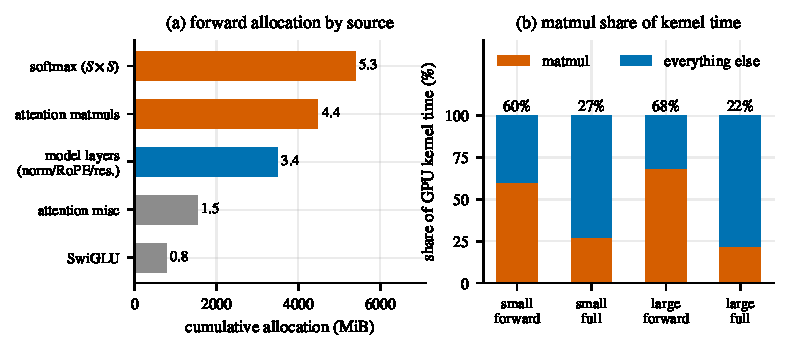
\includegraphics[width=\linewidth]{figures/breakdowns.pdf}
  \caption{(a) Cumulative allocation by source for a medium-model forward pass at context 512 --- softmax intermediates and attention matmuls together account for ${\sim}9.6$ of the 11.4~GiB allocated. (b) Matmul share of GPU kernel time, forward versus full step: the optimizer and backward elementwise kernels dilute matmul's share by a factor of ${\sim}2$--3.}
  \label{fig:breakdowns}
\end{figure}

\subsection{Mixed precision}

Autocast to BF16 \cite{micikevicius2018} (parameters and gradients remain FP32; matmul inputs are downcast) speeds up every model size, and the speedup grows with model size --- 1.83$\times$ (small) to 3.18$\times$ (xl) for forward (Fig.~\ref{fig:mixed}). This is the same effect as the matmul-share measurement above: larger models spend a larger fraction of time in Tensor-Core-eligible matmuls, so lowering their input precision pays off more. Backward speedups are slightly lower (${\sim}2\times$) because its elementwise gradient kernels do not benefit from reduced precision.

BF16 needs no loss scaling (its exponent range matches FP32's), and no NaN or divergence was observed. But precision choice alone does not unblock the largest configuration: xl forward+backward still runs out of memory in bf16, because autocast only reduces the precision of forward activations --- the FP32 master weights, gradients, and optimizer state are untouched. That distinction --- activation precision versus parameter-state residency --- recurs in Sections~\ref{sec:zero} and~\ref{sec:fsdp}.

\begin{figure}[t]
  \centering
  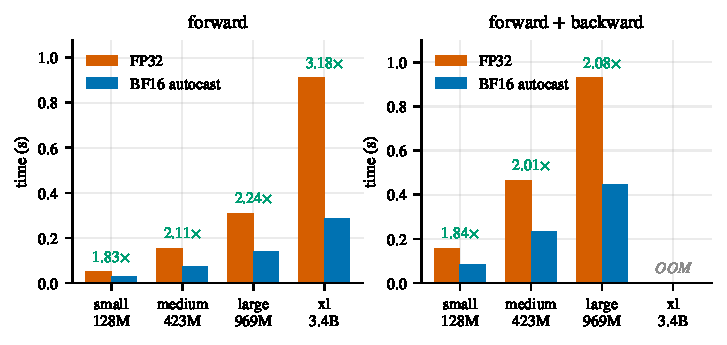
\includegraphics[width=\linewidth]{figures/mixed_precision.pdf}
  \caption{BF16 autocast speedup over FP32, single A6000, context 512. Green labels are the FP32/BF16 time ratio; the xl forward+backward configuration runs out of memory in both precisions.}
  \label{fig:mixed}
\end{figure}

\subsection{Memory}

Peak memory grows ${\sim}4.1\times$ per doubling of context length --- the signature of the $O(S^2)$ attention-score matrix --- and pins the ceiling for FP32 training at a context of 1024 on a 48~GiB card (Fig.~\ref{fig:mem}). Replaying an allocation snapshot shows where the memory goes: for a medium model at context 512, softmax intermediates (5.4~GiB) and the attention matmul outputs (4.4~GiB) account for the vast majority of forward allocations, while the SwiGLU FFN contributes under 1~GiB. The classic memory hierarchy --- parameters, gradients, optimizer state --- is not what caps context length; activation memory is.

\begin{figure}[t]
  \centering
  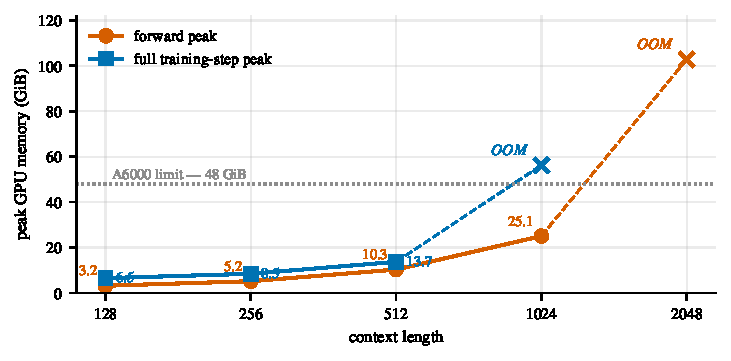
\includegraphics[width=\linewidth]{figures/memory_scaling.pdf}
  \caption{Peak GPU memory versus context length (medium model, batch 4, FP32). Dashed segments extrapolate the measured ${\sim}4.1\times$-per-doubling growth to the configuration where the run actually OOMs; the dotted line is the 48~GiB capacity of an A6000. Forward passes survive to 1024; full training steps stop at 512.}
  \label{fig:mem}
\end{figure}

%=============================================================================
\section{Single-GPU Memory: Residuals and Checkpointing}
\label{sec:memory}
%=============================================================================

\subsection{Autograd residuals and operator fusion}

Backward passes need the forward values they consume, so every operation in a forward pass leaves ``residuals'' in memory. The count is implementation-dependent, and the difference can be large. A plain RMSNorm written as \texttt{x.pow(2).mean(-1).rsqrt()} followed by two multiplies saves \emph{five} tensors for backward, three of them full activation-size; the same computation wrapped in \texttt{torch.compile}, which fuses the five elementwise ops into one, saves \emph{two}. The fused version recomputes intermediates in the backward pass instead of storing them. This is operator fusion --- fewer, larger kernels plus recomputation in exchange for memory --- and it is why production stacks enable \texttt{torch.compile} by default.

\subsection{Gradient checkpointing}

Checkpointing discards activations during forward and recomputes them during backward. The mapping from strategy to memory is not monotonic, and the experiment makes the failure mode concrete (Fig.~\ref{fig:ckpt}):

\begin{itemize}
  \item \emph{Checkpointing everything at once is worse than not checkpointing.} A single checkpoint around all 16 layers peaks at 1.14$\times$ the un-checkpointed memory: the recomputation materializes every layer's residuals simultaneously during backward, so the peak becomes (checkpoint boundaries) $+$ (all residuals).
  \item \emph{Smaller checkpoint blocks are monotonically better here:} block $=$ 4, 2, 1 layers bring the 16-layer peak to 0.52$\times$, 0.42$\times$, 0.37$\times$. Each block boundary costs one activation's worth of memory, each recomputation costs one block's worth of residuals --- the optimum splits the difference.
  \item \emph{Nesting \texttt{torch.utils.checkpoint} calls buys almost nothing.} The nested variant saves only ${\sim}6$\% more than block $=$ 1, because every \texttt{checkpoint(fn, x)} call saves its input tensor for backward; with $N$ nested calls that is $O(N)$ saved boundaries, not $O(\log N)$.
\end{itemize}

The classical analysis \cite{chen2016} explains the shape: for a single-level split into blocks of $K$ layers, peak memory is $\frac{N}{K}C + KC$ (boundaries plus one materialized block) for per-layer residual size $C$, which is minimized at $K=\sqrt{N}$ with peak $2\sqrt{N}C$ and one recomputation per layer. Reaching $O(\log N)$ requires an explicit recomputation \emph{schedule} (Revolve-style \cite{revolve}) that discards boundaries and rebuilds them on demand --- the \texttt{checkpoint} API is a mechanism, not a scheduler.

\begin{figure}[t]
  \centering
  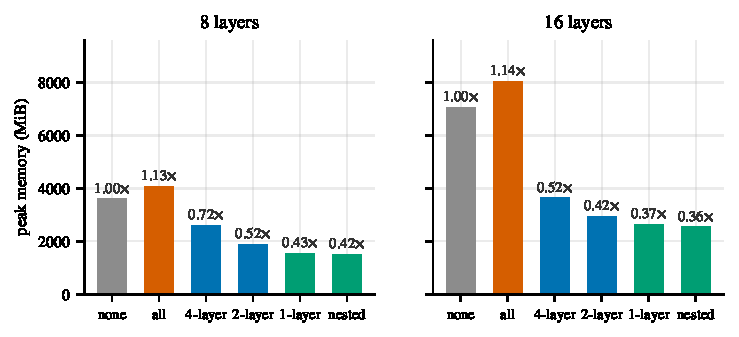
\includegraphics[width=\linewidth]{figures/checkpointing.pdf}
  \caption{Peak memory by checkpointing strategy (medium model, context 512). Labels are relative to the un-checkpointed peak. Checkpointing all layers at once exceeds the baseline; block size 1 is optimal under the single-pass constraint; nesting adds little because the PyTorch API stores one boundary per call.}
  \label{fig:ckpt}
\end{figure}

%=============================================================================
\section{FlashAttention-2}
\label{sec:flash}
%=============================================================================

\subsection{Motivation}

The profiling in Section~\ref{sec:profiling} identifies attention as the outlier on both axes: its softmax is $51\times$ cheaper than matmul in FLOPs yet comparable in time, and its $O(S^2)$ score matrix is the single largest memory consumer. FlashAttention \cite{flash1,flash2} attacks both by never materializing the score matrix: it tiles the computation, keeps tiles in SRAM, and uses an online softmax to accumulate the output.

\subsection{Implementation}

Three implementations were written and tested to pass against a reference attention:

\begin{table}[t]
  \caption{FlashAttention-2 implementation components. All four pass numerical tests against the reference, including causal masking and the tied-weight variant.}
  \label{tab:flash}
  \centering
  \small
  \begin{tabular}{@{}lp{0.64\linewidth}@{}}
    \toprule
    Component & Approach \\
    \midrule
    Forward, PyTorch & Pure-PyTorch online softmax --- numerically exact, used as a reference and as the CPU-runnable test path \\
    Forward, Triton & \texttt{flash\_fwd\_kernel}: one query tile per program, loops over key tiles, rescales the running output accumulator by $\alpha = \exp(m - m_{\text{new}})$; causal masking by skipping/partial-masking key tiles \\
    Backward, compiled & A \texttt{torch.compile}-friendly implementation of the closed-form backward (the standard flash-backward equations), using the saved logsumexp $L$ and the precomputed row-sum $D = \sum (dO \cdot O)$ \\
    Backward, Triton & Two-pass kernels --- one computing $dK, dV$ over key tiles, one computing $dQ$ over query tiles --- so the score matrix is recomputed rather than stored and no atomics are needed \\
    \bottomrule
  \end{tabular}
\end{table}

The core loop (the standard online-softmax recurrence of FlashAttention-2 \cite{flash2}) is:

\begin{algorithm}[t]
  \caption{FlashAttention forward pass with online softmax, for one query tile.}
  \label{alg:flash}
  \begin{algorithmic}[1]
    \Require query tile $Q \in \mathbb{R}^{B_q \times d}$, key/value tiles $\{K_j, V_j\} \in \mathbb{R}^{B_k \times d}$, softmax scale $\tau$
    \Ensure  output tile $O \in \mathbb{R}^{B_q \times d}$, logsumexp $L \in \mathbb{R}^{B_q}$
    \State $m \gets -\infty$; \quad $\ell \gets 0$; \quad $A \gets 0$ \Comment{running max, running sum, accumulator}
    \For{each key tile $(K_j, V_j)$}
      \State $S_j \gets \tau\, Q K_j^{\top}$ \Comment{current scores; consumed and discarded}
      \State $m^{\mathrm{new}} \gets \max\bigl(m,\ \mathrm{rowmax}(S_j)\bigr)$
      \State $\alpha \gets \exp\bigl(m - m^{\mathrm{new}}\bigr)$ \Comment{rescale factor for previously accumulated state}
      \State $\ell \gets \ell\,\alpha + \mathrm{rowsum}\bigl(\exp(S_j - m^{\mathrm{new}})\bigr)$
      \State $A \gets A\,\alpha + \exp\bigl(S_j - m^{\mathrm{new}}\bigr) V_j$
      \State $m \gets m^{\mathrm{new}}$
    \EndFor
    \State $O \gets A / \ell$; \quad $L \gets m + \log \ell$ \Comment{$L$ is stored for the backward pass}
  \end{algorithmic}
\end{algorithm}

Practical notes from writing the Triton kernels: \texttt{tl.dot} requires both operands in the same dtype (the bf16 path needs explicit casts of the probability tile); at head dimension 128 the backward kernel exceeds the shared-memory budget and needs reduced tile sizes with \texttt{num\_stages=1}; and a two-pass backward that recomputes the scores twice is preferable to a one-pass formulation with atomics.

\subsection{Results}

Fig.~\ref{fig:flash} sweeps sequence length from 128 to 65{,}536 across head dimensions and both precisions, comparing flash against a naive PyTorch attention on the same hardware. At head dimension 64, bf16, sequence 65{,}536, flash is 5.7$\times$ faster end-to-end (forward+backward); in FP32 at the same sequence length, the naive implementation runs out of memory while flash completes. Two honest caveats belong here: time still scales as $O(S^2)$ --- flash saves memory, not required computation, as the log-log slope in the figure shows --- and the backward pass is ${\sim}3.5\times$ the forward cost because it recomputes the scores twice.

An Nsight Systems trace at sequence 2048 (bf16) attributes the speedup: naive attention issues 314 kernels for 4.82~ms of GPU time across ${\sim}10$ distinct generic kernels, of which elementwise operations are 50\%, softmax 19\%, and the three separate matmuls 28\%. Flash attention issues 105 kernels for 2.65~ms, and 95\% of that time is in just three purpose-written kernels (forward 25\%, backward $dK$/$dV$ 37\%, backward $dQ$ 33\%). The speedup is therefore attributable to (i) fusion --- a dozen generic kernels became three, (ii) avoided HBM round-trips for the $S^2$ score matrix, and (iii) fewer kernel launches.

\begin{figure}[t]
  \centering
  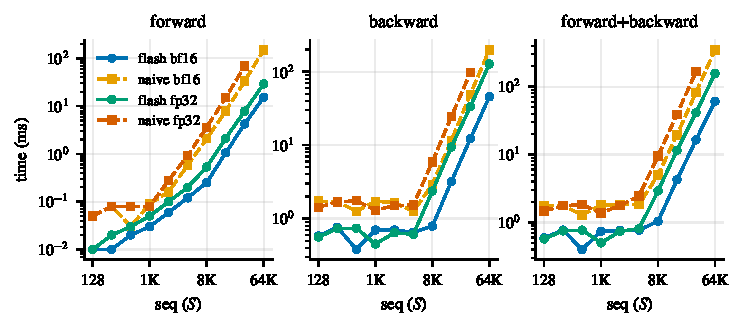
\includegraphics[width=\linewidth]{figures/flash_sweep_d64.pdf}
  \caption{FlashAttention-2 (Triton) versus naive PyTorch attention, head dimension 64, single A6000, from 128 to 65{,}536 tokens (batch 1, causal). Left to right: forward, backward, and forward+backward. The fp32 naive curve ends at 32K --- its 64K point runs out of memory.}
  \label{fig:flash}
\end{figure}

%=============================================================================
\section{Distributed Data Parallel}
\label{sec:ddp}
%=============================================================================

All distributed experiments use \texttt{torch.distributed} with the NCCL backend over the node's PCIe fabric; a gloo/CPU backend is used for correctness tests that must run without GPUs.

\subsection{Characterizing the communication primitive}

An all-reduce sweep over message sizes and world sizes establishes the regime: NCCL all-reduce sustains ${\sim}4.8$~GB/s essentially independent of message size (throughput-linear, i.e.\ bandwidth-bound rather than latency-bound), and going from 2 to 4 ranks inflates the time for a fixed message by ${\sim}4\times$, consistent with the ring all-reduce traffic bound $\frac{N-1}{N}S$. As a sanity check on backends, gloo over TCP is 50--120$\times$ slower than NCCL for the same operation --- fine for logic testing, useless for performance measurement.

\subsection{Three DDP variants}

Three gradient-synchronization schemes were implemented over the same model wrapper:

\begin{itemize}
  \item \emph{Naive}: after backward, all-reduce each parameter's gradient individually (one collective per parameter).
  \item \emph{Flattened}: concatenate all gradients into one buffer and issue a single all-reduce.
  \item \emph{Overlapped}: register a \texttt{post\_accumulate\_grad\_hook} on every parameter; each hook launches an asynchronous all-reduce (\texttt{async\_op=True}) as soon as that parameter's gradient is ready, so communication overlaps the still-running backward pass. A final synchronization joins all pending handles.
\end{itemize}

The flattened variant is the control that isolates \emph{what} the overlap buys: it reduces the number of collective calls from hundreds to one, yet measures identically to naive (790 vs.\ 788~ms per step, Table-equivalent in Fig.~\ref{fig:ddp}) --- with this fabric, launch overhead is negligible and the cost is the bytes moved, not the number of calls. Overlap is the only variant that changes the picture.

\subsection{Results}

Fig.~\ref{fig:ddp} shows the two configurations measured. On 2 GPUs (medium model) the gradient-communication share drops from 43.9\% to 22.6\%, and the step is 14\% faster. On 4 GPUs (large model) the baseline communication share is already 69.4\% --- more ranks and a larger model make the collective more expensive --- and overlap reduces it to 58.6\%, a 13.7\% step-time reduction. The share does not go to zero because the last layers' gradients cannot be sent until the backward pass has produced them; that tail is exposed no matter how early the earlier layers' communication starts. The nsys timeline (Fig.~\ref{fig:timeline}) shows the mechanism directly: in the naive run, NCCL all-reduce occupies long contiguous stretches during which the compute stream is idle (max single all-reduce 93.5~ms); with overlap, the collective is chopped into per-parameter transfers that interleave with compute (max 32.4~ms), and compute kernels occupy a larger share of the timeline.

\begin{figure}[t]
  \centering
  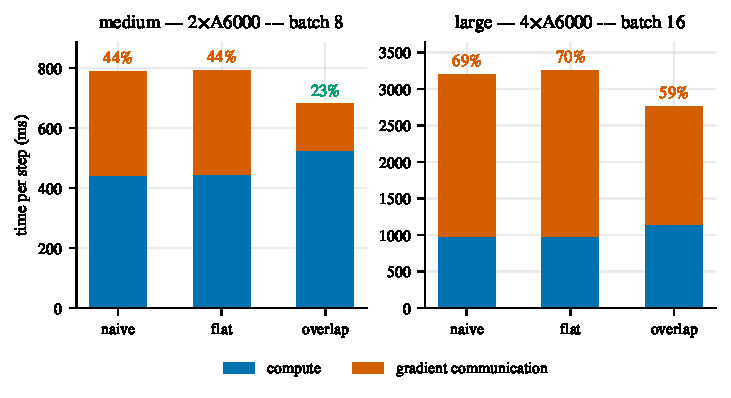
\includegraphics[width=\linewidth]{figures/ddp_variants.pdf}
  \caption{Gradient-communication share and step time for the three DDP variants. Flattening alone changes nothing; overlapping the communication with backward cuts both total time and the communication share.}
  \label{fig:ddp}
\end{figure}

\begin{figure}[t]
  \centering
  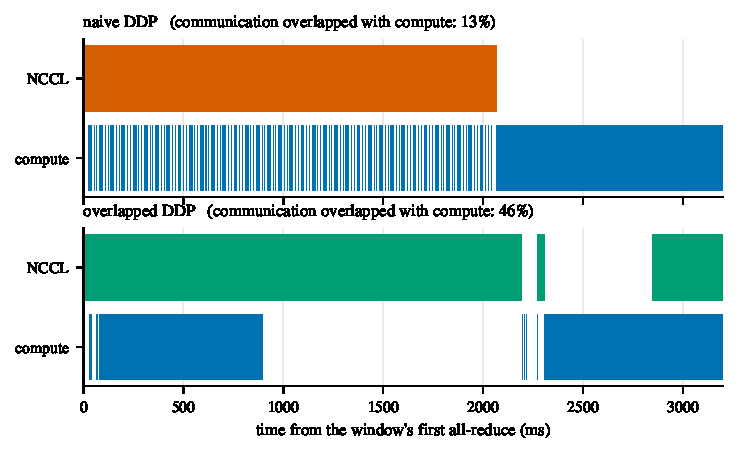
\includegraphics[width=\linewidth]{figures/nsys_timeline.pdf}
  \caption{Kernel occupancy timelines reconstructed from the Nsight Systems exports (large model, 4 GPUs, rank 0), one 3.2~s window per variant starting at the window's first all-reduce. Top row of each panel: NCCL kernels; bottom row: all other kernels (compute). Naive DDP funnels every gradient into long contiguous collectives during which the GPU computes nothing; the overlapped variant issues per-parameter transfers that interleave with the backward pass, raising the share of communication overlapping with compute from 13\% to 46\% of the window.}
  \label{fig:timeline}
\end{figure}

%=============================================================================
\section{Optimizer-State Sharding (ZeRO-1)}
\label{sec:zero}
%=============================================================================

Optimizer state is a fixed cost: AdamW keeps two FP32 moments per parameter, so a DP replica pays $3\times$ parameter memory in weights plus optimizer state alone, independent of batch size. Sharding it is the idea behind ZeRO stage 1 \cite{zero}: each rank owns $1/N$ of the parameters and their optimizer state, computes updates only for its shard, and broadcasts updated parameters afterward.

The implementation wraps any \texttt{torch.optim.Optimizer}: parameters are partitioned by \emph{index} (not \texttt{id()}, which is process-local and differs across ranks --- using the object id produces silent mismatches or deadlocks), each rank constructs a real optimizer over its shard, and \texttt{step()} is followed by a broadcast of owned parameters.

\begin{table}[t]
  \caption{Optimizer-state sharding, medium model, 2 GPUs. The saving is 23.7\%, not the 50\% a ``half the state'' estimate suggests, because only optimizer state is sharded: weights, gradients, and activations are replicated.}
  \label{tab:zero}
  \centering
  \small
  \begin{tabular}{@{}lrr@{}}
    \toprule
    Metric & DDP & ZeRO-1 \\
    \midrule
    Memory before step & 6479~MiB & 4942~MiB \\
    Memory after step  & 6479~MiB & 4943~MiB \\
    Memory reduction   & ---       & \textbf{23.7\%} \\
    Step time          & 548.8~ms  & 626.5~ms \\
    Time overhead      & ---       & \textbf{+14.2\%} \\
    \bottomrule
  \end{tabular}
\end{table}

Two numbers deserve comment. The reduction is 23.7\% rather than ${\sim}50$\% of total memory because activations, gradients, and weight traffic are untouched --- sharding removes $2P$ bytes of moments and leaves everything else, so the fraction depends on how much of the total the moments are. The 14.2\% time overhead is the price of the post-step broadcast, paid on every step; it shrinks relative to compute as models grow, but it is the reason sharding depth matters: nothing is gained by moving state off a rank if the same bytes must be broadcast back.

%=============================================================================
\section{Fully-Sharded Data Parallel}
\label{sec:fsdp}
%=============================================================================

ZeRO-1 shards optimizer state; FSDP \cite{fsdp} shards the weights themselves. Each rank stores $1/N$ of each \texttt{Linear}/\texttt{Embedding} weight, all-gathers the full weight just before the layer's forward, drops it after use, all-gathers again for the backward, and reduce-scatters the (row) gradients back to the owning ranks so no rank ever holds more than $1/N$ of the gradient. Norm parameters, which are small and needed in full, keep plain all-reduced gradients.

\subsection{Implementation notes}

Four non-obvious issues surfaced, all of which are the kind of thing that separates a toy from a working implementation:

\begin{itemize}
  \item A row slice's \texttt{.contiguous()} is a no-op --- it returns a \emph{view} of the full tensor, so the shard silently retains the whole weight. Shards must be \texttt{.clone()}d.
  \item Under gloo, all-gathering a weight that requires grad triggers an autograd error (``view created in no\_grad'') because the collective is not autograd-aware. Wrapping the communication in \texttt{torch.no\_grad()} fixes it.
  \item \texttt{all\_gather\_into\_tensor} (the single-output form) avoids a deadlock that a list-of-tensors all-gather plus \texttt{cat} produced on this PCIe topology: the cat kernel can read the NCCL output on the wrong stream.
  \item NCCL runs on its own stream; a \texttt{torch.cuda.synchronize()} (or proper stream dependency) is required after each collective before the gathered weight is used by default-stream compute, or the run deadlocks.
\end{itemize}

Gradients are divided by world size after reduction so that per-rank losses average to the global mean, and \texttt{compute\_dtype} downcasts the gathered weight for compute while the master shard stays FP32 --- the standard ``sharded weights, mixed-precision compute'' arrangement.

\subsection{Results and cross-validation}

On the small model with 2 GPUs, FSDP reduces steady-state memory by 43.0\% --- close to the theoretical $1/N=50$\% bound, with the residue being the un-sharded parts (norms, buffers, the optimizer's own state holders). Peak memory, however, is 7.1\% \emph{higher} than the non-sharded baseline. The reason is instructive: this simplified implementation materializes the full weight during the forward and keeps it alive for backward (\texttt{save\_for\_backward}), so the peak contains the shard, the full weight, activations, and gradients simultaneously. Production FSDP avoids this by prefetching the next layer's gather --- holding two full weights at once but releasing each immediately after use --- and by overlapping the gather with compute; our serialized collectives on a PCIe fabric cannot hide that cost. \emph{Steady-state savings are the right measure of sharding; peak savings are a measure of the memory schedule.}

To validate the from-scratch implementation, the same model was trained with PyTorch's official \texttt{DistributedDataParallel}, \texttt{ZeroRedundancyOptimizer}, and \texttt{FullyShardedDataParallel} (FULL\_SHARD) under identical conditions (Fig.~\ref{fig:hier}). The steady-state memory ordering is exactly as theory predicts --- DDP 983~MiB, ZeRO-1 492~MiB, FSDP 246~MiB --- and the from-scratch FSDP lands at 281~MiB, within 14\% of the official implementation. The residual gap and the higher steady number both come from the missing prefetch/release discipline noted above. Peak memory differs far less across the three (5638/4653/4894~MiB) because at this scale activations dominate the peak in every configuration.

\begin{figure}[t]
  \centering
  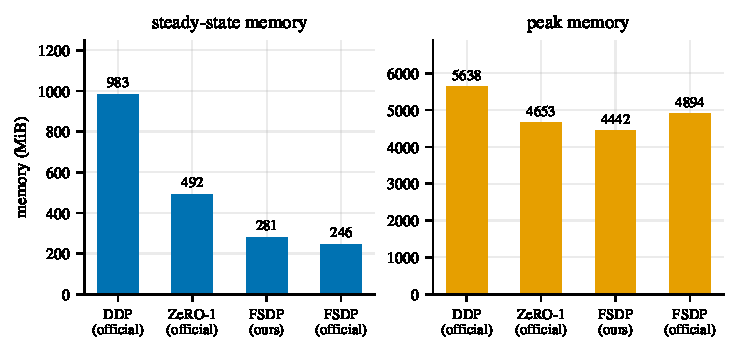
\includegraphics[width=\linewidth]{figures/memory_hierarchy.pdf}
  \caption{Steady-state and peak memory for official PyTorch DDP, ZeRO-1 (\texttt{ZeroRedundancyOptimizer}), and FSDP, together with the from-scratch FSDP of this report (small model, 2 GPUs, gloo). Steady-state memory falls by the expected $2\times$ per stage; peaks are dominated by activations and move much less.}
  \label{fig:hier}
\end{figure}

%=============================================================================
\section{Analytical Scaling Limits}
\label{sec:analysis}
%=============================================================================

The measured regime --- communication-bound at 4 GPUs on PCIe --- motivates the question of where the limits are. Using a ring-communication model with per-device egress bandwidth $W$ and per-device compute $C$, all-gather and reduce-scatter of $S$ bytes cost $\frac{N-1}{N}\frac{S}{W}$, and all-reduce costs twice that. For a SwiGLU FFN block with batch $B$, model width $D$, and hidden width $D_{\text{ff}}$ (the tensor-parallel decomposition follows Megatron-LM \cite{megatron}):

\begin{table}[t]
  \caption{Scaling conditions for the four strategies (standard derivations from the ring-communication cost model of the text). $N$ is the number of devices. The tensor-parallel condition shown is the stricter backward-pass one; the forward-pass condition has $3D_{\text{ff}}W/(2C)+1$ in its place.}
  \label{tab:scaling}
  \centering
  \small
  \begin{tabular}{@{}lcc@{}}
    \toprule
    Strategy & Non-bottleneck condition & Communication \\
    \midrule
    Data parallel & $N > BW/C + 1$ & gradient all-reduce \\
    FSDP & $N > BW/C + 1$ & weight all-gather + grad reduce-scatter \\
    Tensor parallel & $N > 3D_{\text{ff}}W/C + 1$ & activation all-reduce per pass \\
    FSDP + TP, no overlap & $N \le 3BD_{\text{ff}}W^2/(8C^2)$ & the two above, summed \\
    FSDP + TP, overlapped & $N \le 3BD_{\text{ff}}W^2/(2C^2)$ & the two above, overlapped \\
    \bottomrule
  \end{tabular}
\end{table}

The data-parallel and FSDP conditions share the form $N > BW/C + 1$: doubling bandwidth-per-FLOP (a faster fabric) or halving the batch moves the crossover, which is the formal statement of ``communication-bound on PCIe'' that the DDP measurements exhibit. The most interesting result is the two-dimensional FSDP+TP case. Without overlap between the FSDP gather and the TP all-reduce, devices scale only up to $3BD_{\text{ff}}W^2/(8C^2)$; allowing the two communication phases to overlap raises the bound to $3BD_{\text{ff}}W^2/(2C^2)$ --- exactly $4\times$ more devices. Communication/computation overlap, which Section~\ref{sec:ddp} bought for a 13.7\% step-time reduction here, is worth a factor of four in maximum scale.

%=============================================================================
\section{Lessons Learned}
%=============================================================================

\begin{itemize}
  \item \emph{Measure before optimizing.} The profile changed the plan twice: the softmax/FLOP ratio pointed at attention before any kernel was written, and the ``checkpointing all layers is worse than nothing'' result was not expected from the textbook description alone.
  \item \emph{FLOPs are not time.} Matmul holds over 60\% of forward FLOPs and under 30\% of a full step's kernel time. Precision and fusion decisions should follow time and byte traffic, not operation counts.
  \item \emph{The bottleneck moves as you fix things.} Activations cap context length; optimizer state caps batch size per replica; communication caps device count. Each optimization in this report relocates the bottleneck rather than removing it.
  \item \emph{Overlap is the only DDP lever that matters here.} Flattening collectives changed nothing measurable; issuing them during the backward pass changed everything. The bytes, not the calls, are the cost on this fabric.
  \item \emph{Steady-state and peak memory are different problems.} FSDP's 43\% steady-state reduction coexists with a higher peak, because the peak is a scheduling artifact (when the full weight is alive) rather than a capacity one.
  \item \emph{Correctness first, then the fabric.} Sharded optimizers and FSDP both failed on rank-stable identity (index vs.\ \texttt{id()}) and stream ordering long before bandwidth mattered. The gloo/CPU path that made these components testable without GPUs was the highest-leverage piece of infrastructure in the whole project.
\end{itemize}

%=============================================================================
\section{Reproducibility}
%=============================================================================

The complete implementation and experiment scripts are in the repository's \texttt{lm\_systems/} module. Measurements in this report were produced by: \texttt{benchmark.py} (timed training steps; \texttt{--precision bf16}, \texttt{--memory-profile}), \texttt{profile\_attention.py} and \texttt{nsys\_attn\_compare.py} (kernel attribution), \texttt{flash\_attention.py} with \texttt{flash\_benchmark.py} (attention correctness and the 80-configuration sweep), \texttt{ddp.py} with \texttt{ddp\_benchmark.py} (three DDP variants), \texttt{sharded\_optimizer.py} and \texttt{fsdp.py} with their accounting scripts, and \texttt{official\_dist\_benchmark.py} (the PyTorch official-implementation comparison). Correctness for the distributed components is covered by the test-suite adapters (\texttt{tests/adapters.py}), run over gloo/CPU and re-run five times to expose races. Figures in this report were generated from the raw measurement logs by \texttt{report/make\_figures.py}.

\vspace{0.8em}
\noindent\rule{\linewidth}{0.4pt}
\vspace{-0.4em}
\begin{quote}
\small \emph{Acknowledgement of scope.} This report is an implementation and measurement study: the component specifications (FlashAttention-2 tiling, the parallel scaling analysis, the model configurations) follow the published work cited throughout. The implementations, measurement protocol, experiments, and all results in this report are my own; a reference test suite was used as a correctness oracle throughout.
\end{quote}

\begin{thebibliography}{9}

\bibitem{chen2016}
Tianqi Chen, Bing Xu, Chiyuan Zhang, and Carlos Guestrin.
\newblock Training deep nets with sublinear memory cost.
\newblock \emph{arXiv:1604.06174}, 2016.

\bibitem{flash1}
Tri Dao, Daniel Y. Fu, Stefano Ermon, Atri Rudra, and Christopher R\'e.
\newblock FlashAttention: Fast and memory-efficient exact attention with IO-awareness.
\newblock \emph{NeurIPS}, 2022.

\bibitem{flash2}
Tri Dao.
\newblock FlashAttention-2: Faster attention with better parallelism and work partitioning.
\newblock \emph{arXiv:2307.08691}, 2023.

\bibitem{fsdp}
Yanli Zhao, Andrew Gu, Rohan Varma, Liang Luo, Quanzheng Li, Min Xu, Less Wright, Hamid Shojanazeri, Myle Ott, Sam Shleifer, Alban Desmaison, Can Balioglu, Pritam Damania, Bernard Nguyen, Geeta Chauhan, Yuchen Hao, Ajit Mathews, and Shen Li.
\newblock PyTorch FSDP: Experiences on scaling fully sharded data parallel.
\newblock \emph{Proceedings of the VLDB Endowment}, 2023.

\bibitem{megatron}
Mohammad Shoeybi, Mostofa Patwary, Raul Puri, Patrick LeGresley, Jared Casper, and Bryan Catanzaro.
\newblock Megatron-LM: Training multi-billion parameter language models using model parallelism.
\newblock \emph{arXiv:1909.08053}, 2019.

\bibitem{micikevicius2018}
Paulius Micikevicius, Sharan Narang, Jonah Alben, Gregory Diamos, Erich Elsen, David Garcia, Boris Ginsburg, Michael Houston, Oleksii Kuchaiev, Ganesh Venkatesh, and Hao Wu.
\newblock Mixed precision training.
\newblock \emph{ICLR}, 2018.

\bibitem{revolve}
Andreas Griewank and Andrea Walther.
\newblock Algorithm 799: Revolve --- an implementation of checkpointing for the reverse or adjoint mode of computational differentiation.
\newblock \emph{ACM Transactions on Mathematical Software}, 2000.

\bibitem{zero}
Samyam Rajbhandari, Jeff Rasley, Olatunji Ruwase, and Yuxiong He.
\newblock ZeRO: Memory optimizations toward training trillion parameter models.
\newblock \emph{SC20: International Conference for High Performance Computing, Networking, Storage and Analysis}, 2020.

\end{thebibliography}

\end{document}
